\section{Evaluation}
%To evaluate our proposed streaming system, 
We compare the performance of FLSD with two different streaming systems --  {\it Simple} and {\it DHT based}. The {\it Simple} environment emulates the DASH based client-server adaptive streaming where we have used three baselines -- BOLA~\cite{bola2-acm-mmsys2018}, MPC~\cite{MPC-SIGCOMM-2015} and Pensieve~\cite{Pensieve}.  The {\it DHT} environment represents an environment with a distributed hash table (DHT) based peer-to-peer system \cite{shen2013dht}.
%\notesc{Give a citation for DHT.} 
All the above streaming clients have been implemented in Python; the source code of the implementation is publicly available at \url{https://github.com/abhimp/FLSD}.
% and has been executed over an emulation environment as discussed next. 
%Our proposed algorithm is based on collaborative segment downloading. It important to have a large set of players in the network, otherwise it falls back as a standalone player with BOLA as the ABR. It is difficult to have such a big network in a real environment, and it is more difficult to configure such a big network with different network condition. To avoid all these issues, we emulate the streaming player on top of a simulated environment.
\subsection{Emulation Environment}
\label{sec:simulatorprop}
We have developed an emulator platform similar to~\cite{Pensieve} to analyze the performance of FLSD. In the emulation platform, all the players in the system have access to system clock which is an event-driven clock handled by the emulator core. The emulator uses a reference network to define the connectivity across the networked nodes; where every node of the network runs a streaming player. %The network characteristics of the reference network has been used to configure the network characteristics of the emulated network. 
We maintain a global playback time defined by the live streaming server, and the streaming server generates DASH segments of a live video based on the global playback time, maintaining the video frame recording timestamps. We use Mahimahi \cite{mahimahi} network traces to emulate the network condition of the links between the streaming server and the players, where we randomly assign different Mahimahi traces to every player in a network. The emulated player can use any existing ABR implementation without any modification as long as it takes the player-state as the input and gives the next segment quality as the output. 
%	\item The simulator can emulate a network if it runs with a reference network. It places a player per node of the reference network.
%	\item Any Two players in the system communicate only through the emulated network. For the emulated network, simulator needs a reference network which will provide the bandwidth delay between two nodes. We calculate communication delay carefully and a conservative way so that it does not violets the real communications between delay. For TCP like communication between two play in the simulated network, we calculate the transmission time based the delay and sender buffer. It is not accurate, but it gives higher transmission time than our empirical studies.
%	\item A player will never access the future video information. We maintain a global playback time. The video server module will never reveal any informations about a segment unless that segment can be downloaded according to the global playback time.
%	\item We use Mahimahi \cite{mahimahi} like network trace to simulate the network condition of the links between video server to a player. We randomly assigned different Mahimahi traces to every player in a network.
%	\item The emulated player can use any existing ABR implementation without any modification as long as it takes the player state as input and gives next segment quality as the output. This feature eliminates the possibility of faulty implementation.
%\end{itemize}
In the emulated environment, we use Eq.~(\ref{eqn:transmissionTime}) to compute the transmission time $T_{ij}$ between two players $P_i$ and $P_j$ in a coalition. Here $clen$ is the data length of the video segment, $d_{ij}$ is delay between two nodes, $buf$ is the sender buffer and $z$ is the noise factor which is uniformly distributed between $\theta_1$ to $\theta_2$. 
%\notesc{What is $P(x)$?}
\begin{align}
T_{ij} = clen\times \frac{buf}{2\times d_{ij}} \times z \mbox{\hspace{1cm}}& \theta_1 <= z <= \theta_2  
%& \mathcal{p}(x) = \frac{1}{\theta_2 - \theta_1} 
\label{eqn:transmissionTime}
\end{align}
%
%\begin{figure}[ht]
%	\captionsetup[subfigure]{}
%	\begin{center}
%		\subfloat[\label{fig:avgBitratebox} Averge Bitrate]{
%			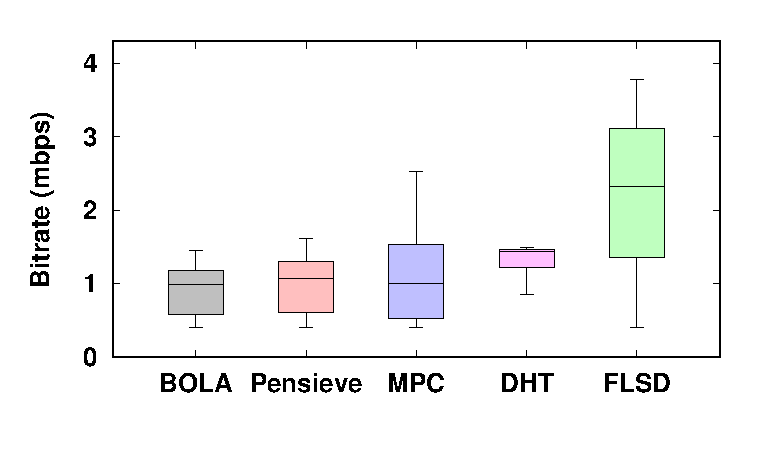
\includegraphics[width=0.49\linewidth]{img/grpbasic/avgbitrate_box_1}
%		}
%		\subfloat[\label{fig:avgBitratecmf}Average Bitrate]{
%			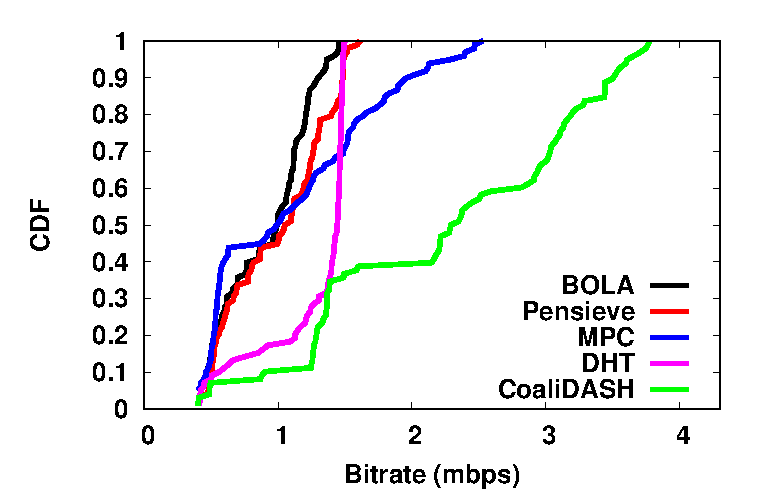
\includegraphics[width=0.49\linewidth]{img/grpbasic/avgbitrate_cdf_1}
%		}
%	\end{center}
%	\caption{\label{fig:avgBitrate} Average bitrate played}
%\end{figure}
%\begin{figure}[ht]
%	\captionsetup[subfigure]{}
%	\begin{center}
%		\subfloat[\label{fig:avgBitrateVarbox}]{
%			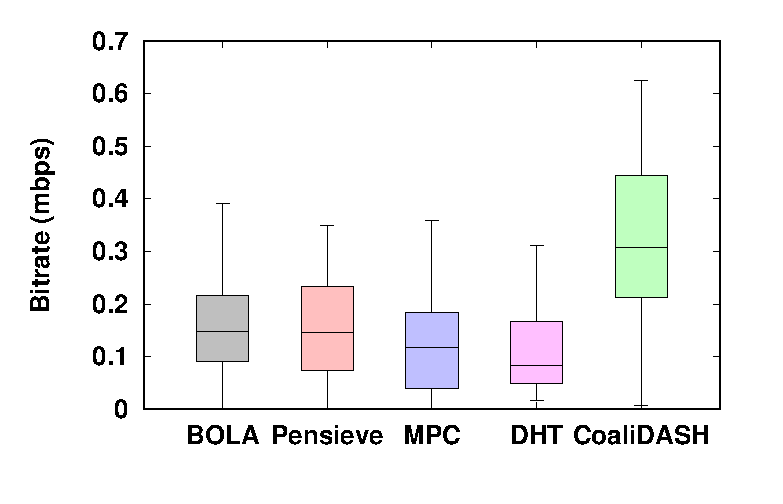
\includegraphics[width=0.49\linewidth]{img/grpbasic/avgbitrate_var_box_1}
%		}
%		\subfloat[\label{fig:avgBitrateVarcmf}]{
%			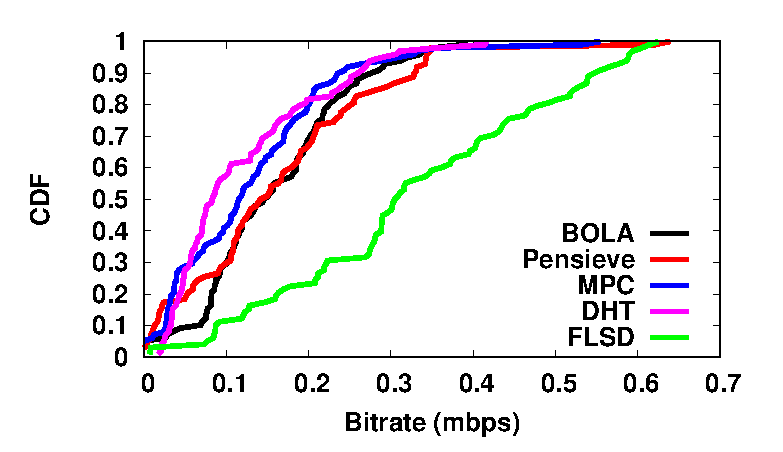
\includegraphics[width=0.49\linewidth]{img/grpbasic/avgbitrate_var_cdf_1}
%		}
%	\end{center}
%	\caption{\label{fig:avgBitrateVar} Average bitrate variation during playback}
%\end{figure}
%As we discussed at \ref{sec:simulatorprop}, we designed all this environment carefully so that it emulates real network condition and does not take any unfair advantage of the fact that everything is directly accessible. We use BOLA as the base ABR for every environment if not specified otherwise. We compared our system with BOLA, MPC and Pensieve ABR. We use the implementation provided by Pensieve source code directly for BOLA, MPC and Pensieve. The {\it Simple} environment was used as the environment while experimenting with BOLA, MPC and Pensieve. Although we run experiments with both RobustMPC, we have shown only RobustMPC results of RobustMPC as results are almost the same. As BOLA, MPC and Pensieve are ABR for the single player streaming system, we implement DHT as a baseline of the peer-to-peer system.
\subsection{Experimental Setup}
We run our emulation with a large set of autonomous system data available from SNAP database~\cite{ASDataSet} as reference networks. We have executed the systems over 710 reference networks, with 100 to 1000 nodes per network. As mentioned earlier, every network node runs a streaming client. To train the model for learning based adaptive streaming like Pensieve~\cite{Pensieve}, we use $58$ DASH-ified videos with a total duration of $45$ hours. We have taken only lengthy videos for our experiment because most of the live online live streaming lasts more than one hour\footnote{\url{https://50wheel.com/the-top-video-live-streaming-statistics-to-know-in-2018/} (Accessed: \today)}. We have created Mahimahi compatible traces from publicly available dataset, like a broadband trace from FCC~\cite{dataset-fcc} and the 3G/HSDPA mobile dataset collected in Norway~\cite{dataset-norway}. We modified these datasets as described in \cite{Pensieve} to make it Mahimahi compatible.

For experimentation, we use the QoE definition as given in \cite{Pensieve}. According to this definition, we consider three QoE components -- (i) average quality level, (ii) average jump in the quality level (smoothness of the video playback) and (iii) re-buffering time. Let $\mathcal{Q}_n$ denote the quality level for video segment $n$ and $\mathcal{T}_n$ be the re-buffering time. Considering that there are $N$ number of segments in a reference video, the average QoE is defined as follows. 
\begin{equation}
QoE = \frac{\alpha}{N}\sum_{n=1}^{N} \mathcal{F}(\mathcal{Q}_n) - \frac{\beta}{N-1} \sum_{n=2}^{N}\lvert\mathcal{F}(\mathcal{Q}_n) -\mathcal{F}(\mathcal{Q}_{n-1})\rvert - \gamma\mathcal{T}_n
\label{eqn:QoE}
\end{equation}
Here, $\alpha$, $\beta$ and $\gamma$ are weight factors (values between 0 and 1) to individual components, such that $\alpha + \beta + \gamma = 1$. 
%\begin{figure}[h]
%	\captionsetup[subfigure]{}
%	\begin{center}
%		\subfloat[\label{fig:Stall_Timebox}]{
%			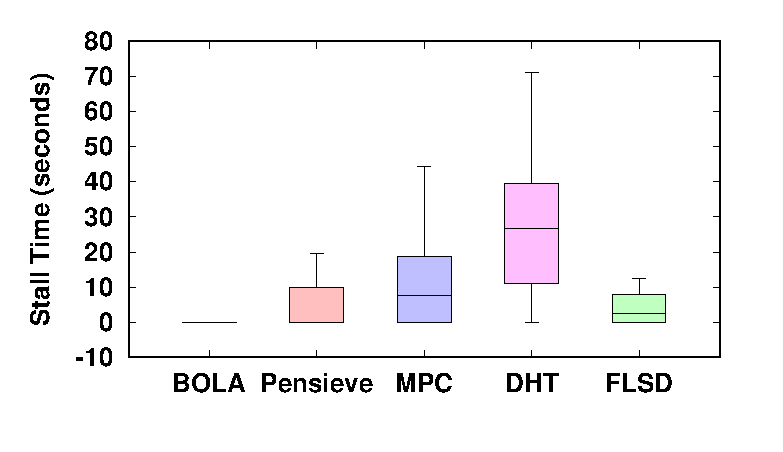
\includegraphics[width=0.49\linewidth]{img/grpbasic/stalltime_box_1}
%		}
%		\subfloat[\label{fig:Stall_Timecmf}]{
%			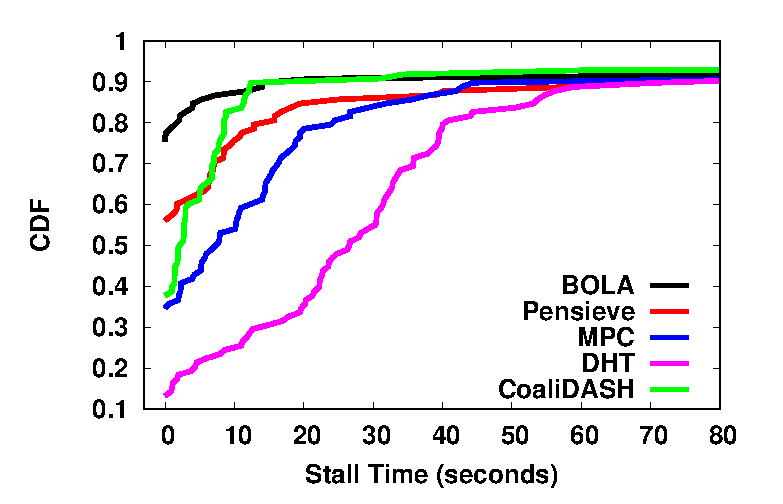
\includegraphics[width=0.49\linewidth]{img/grpbasic/stalltime_cdf_1}
%		}
%	\end{center}
%	\caption{\label{fig:Stall_Time}Total stall time observed each player}
%\end{figure}
%
%\begin{figure}[h]
%	\captionsetup[subfigure]{}
%	\begin{center}
%		\subfloat[\label{fig:QoEbox}]{
%			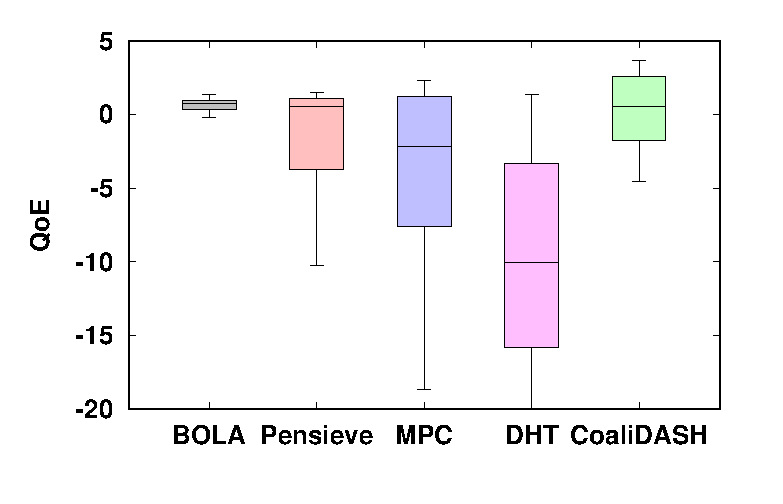
\includegraphics[width=0.49\linewidth]{img/grpbasic/qoe_box_1}
%		}
%		\subfloat[\label{fig:QoEcmf}]{
%			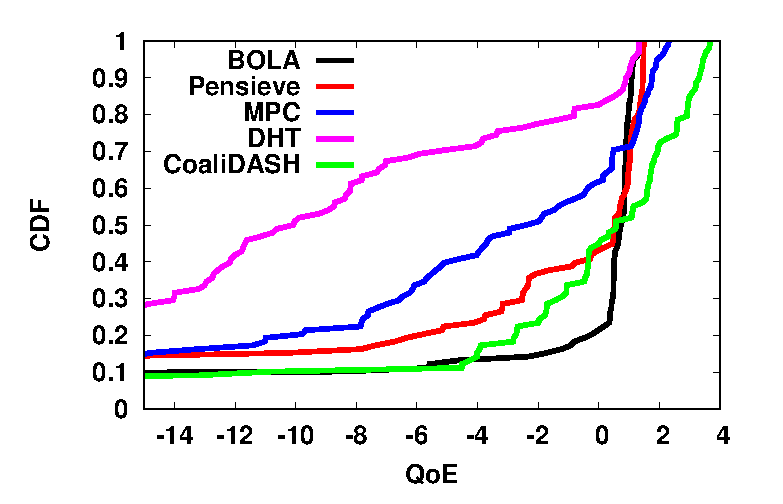
\includegraphics[width=0.49\linewidth]{img/grpbasic/qoe_cdf_1}
%		}
%	\end{center}
%	\caption{\label{fig:QoE}Quality of experience (linear)}
%\end{figure}
\begin{figure}[ht]
	\captionsetup[subfigure]{}
	\begin{center}
		\subfloat[\label{fig:avgBitratecmf}Average Bit-rate]{
			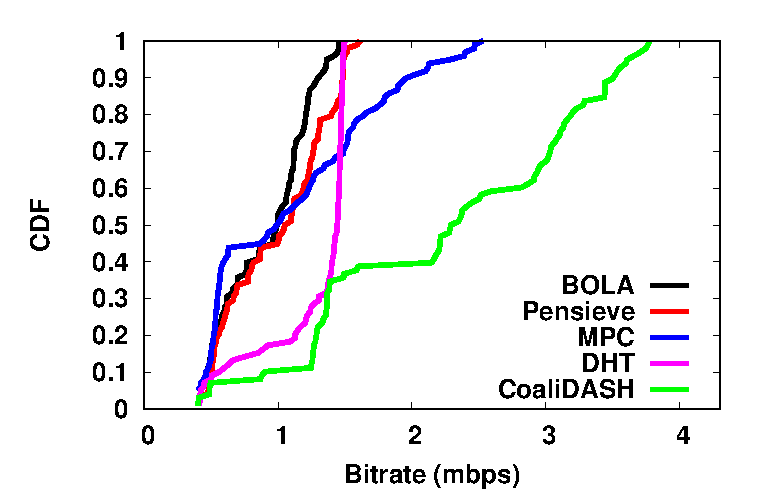
\includegraphics[width=0.49\linewidth]{img/grpbasic/avgbitrate_cdf_1}
		}
     	\subfloat[\label{fig:avgBitrateVarcmf}Bit-rate Variation]{
     			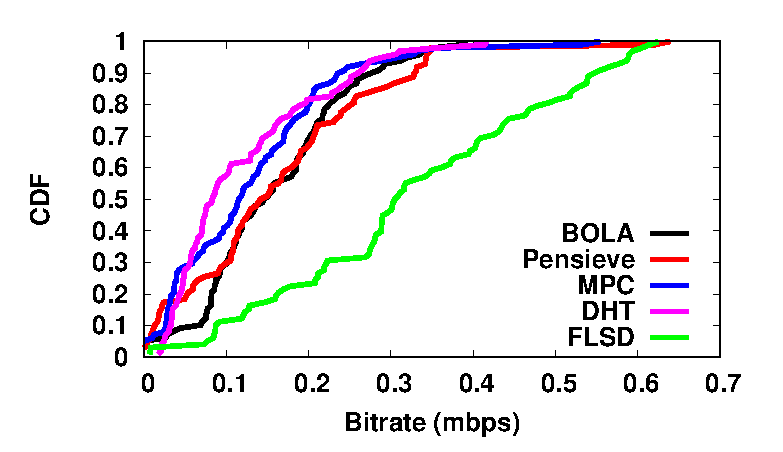
\includegraphics[width=0.49\linewidth]{img/grpbasic/avgbitrate_var_cdf_1}
     		}
	\end{center}
	\caption{\label{fig:avgBitrate} QoE Components: Average Bit-rate and Bit-rate Variation}
\end{figure}
\subsection{Results}
We first observe the individual QoE components for FLSD in comparison with other baselines. Fig.~\ref{fig:avgBitratecmf} compares the average playback bit-rate for various streaming applications. In Fig.~\ref{fig:avgBitrateVarcmf}, we show the variation in average playback bit-rates, which indicate the smoothness of the video rendering. We observe that the performance of BOLA in terms of average playback bit-rate is very low, and most of the players played the videos in lower average quality compared to other baselines. BOLA is very conservative about the bitrate, whereas it is much concerned about the re-buffering time. Pensieve and MPC improve the video quality compared to BOLA by utilizing reinforcement learning and deep inspection, respectively. DHT is the first system which uses the knowledge of existing players in the network and form a peer-to-peer architecture for collectively download the videos. So, it improves the average video quality compared to client-server based ABR. However, FLSD clusters the players based on their network conditions and render the videos keeping the coalition members in sync. In Fig.~\ref{fig:avgBitratecmf}, it is clear that there are clusters of players who play a video in almost equal quality levels. Although we observe that the average variation in the video quality is higher for FLSD; however, it is because the deviation of video quality levels among various coalitions. In a coalition where majority of the members have low network resources, the average quality of the video gets drop down. 
%A slight change in the quality incurs high variation.
\begin{figure}[!ht]
	\captionsetup[subfigure]{}
	\begin{center}
		\subfloat[\label{fig:Stall_Timecmf}Total Re-buffering Time]{
			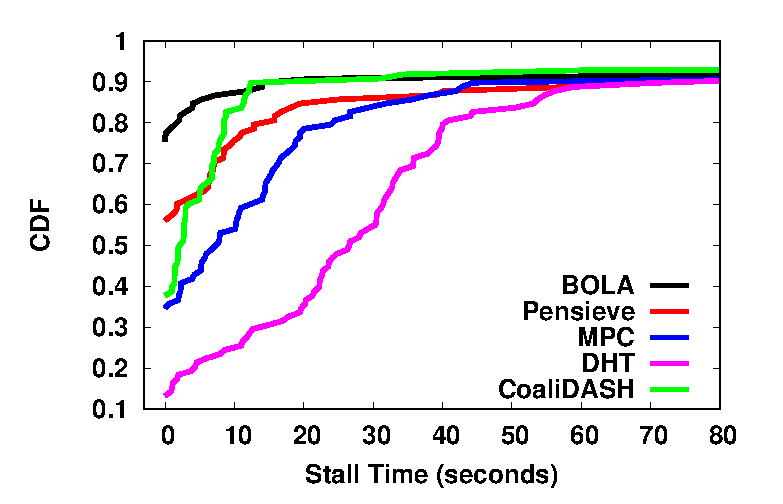
\includegraphics[width=0.49\linewidth]{img/grpbasic/stalltime_cdf_1}
		}
       	\subfloat[\label{fig:QoEcmf}Overall QoE]{
       			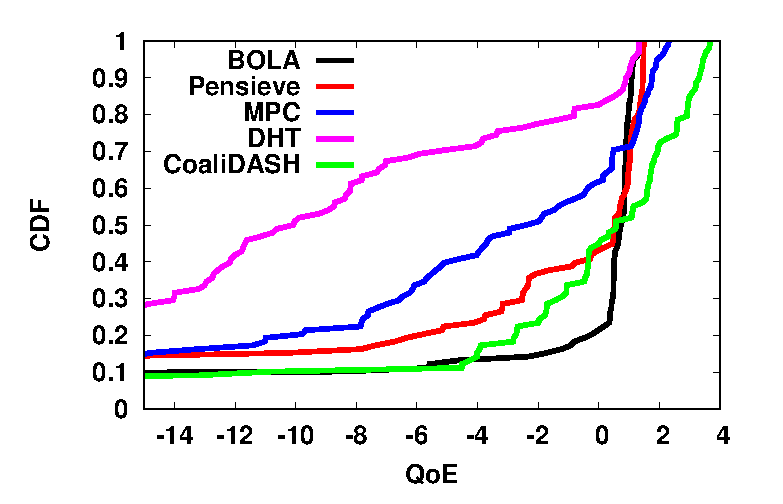
\includegraphics[width=0.49\linewidth]{img/grpbasic/qoe_cdf_1}
       		}
	\end{center}
	\caption{\label{fig:avgBitrateVar} Re-buffering Time and Overall QoE}
\end{figure}
Next, Fig.~\ref{fig:Stall_Timecmf} compares the total re-buffering time among various baselines. We observe that the re-buffering time is very high for DHT because it needs more time to search for a video segment from the network before it can fetch it directly from the streaming server. The re-buffering time for FLSD is moderated although it includes the skip time during the synchronization among the members of the coalition. BOLA incurs almost no re-buffering time; whereas Pensieve and MPC suffer from noticeable re-buffering time. As the re-buffering time is a significant contributor in the overall QoE measurement (Eq.~(\ref{eqn:QoE})), the overall QoE for various baselines, as shown in Fig.~\ref{fig:QoEcmf}, indicates that FLSD outperforms other baselines in term of maximum achievable QoE.  Among the various scenarios simulated over our developed platform, more than $50\%$ of the cases, FLSD incurs a high QoE (value between $2$--$4$). 
\begin{figure}[!ht]
	\captionsetup[subfigure]{}
	\begin{center}
		\subfloat[\label{fig:cdnuploaded_byte} Data downloaded from server]{
			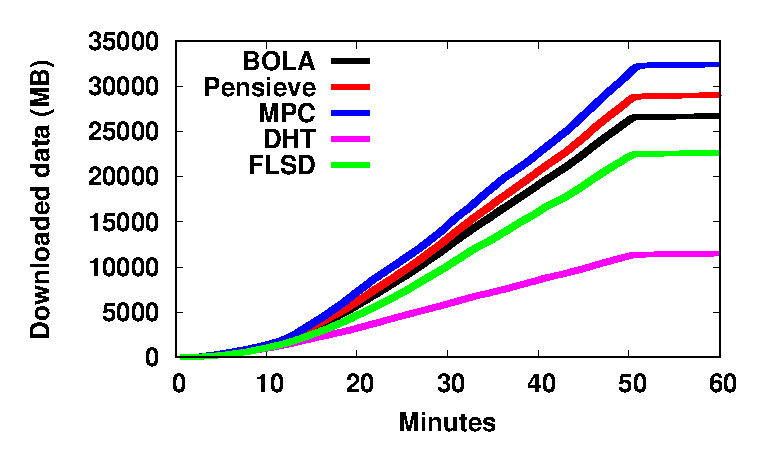
\includegraphics[width=0.49\linewidth]{img/grpbasic/cdnupload_1}
		}
		\subfloat[\label{fig:cdnuploaded_cnt} Segment downloads from server]{
			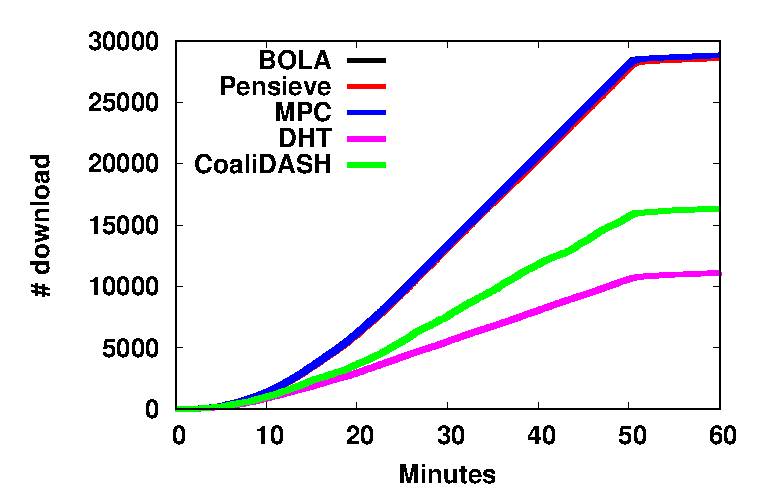
\includegraphics[width=0.49\linewidth]{img/grpbasic/cdnuploadcnt_1}
		}
	\end{center}
	\caption{\label{fig:cdnuploaded}Streaming Server Usage}
\end{figure}
\begin{figure*}[!ht]
	\captionsetup[subfigure]{}
	\begin{center}
		\subfloat[\label{fig:grp_qoe}Overall QoE]{
			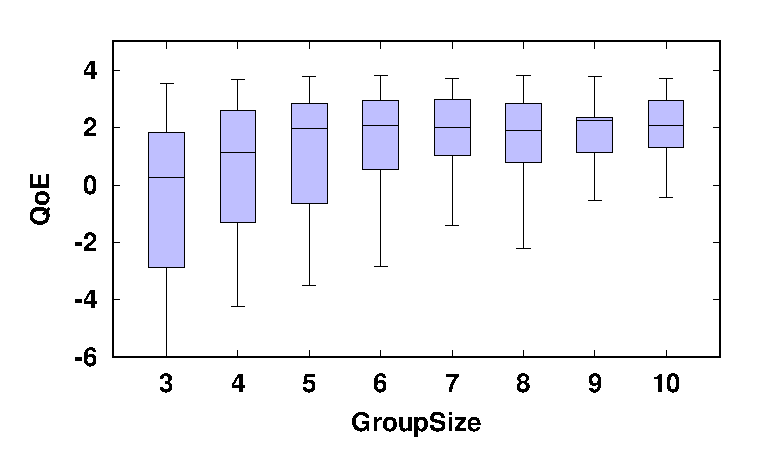
\includegraphics[width=0.49\linewidth]{img/grpbasic/grpsz_qoe}
		}
		\subfloat[\label{fig:grp_download}Amount of Data Upload and Download]{
			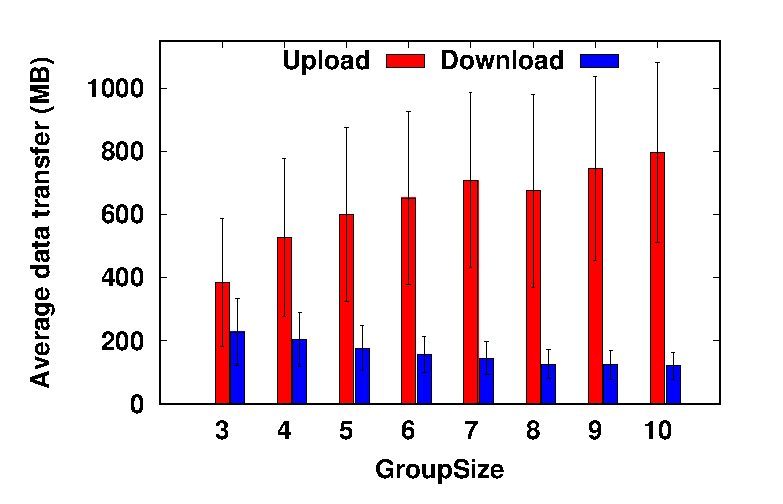
\includegraphics[width=0.49\linewidth]{img/grpbasic/grpsz_upload_download}
		}
	
		\subfloat[\label{fig:grp_fairness}Fairness]{
			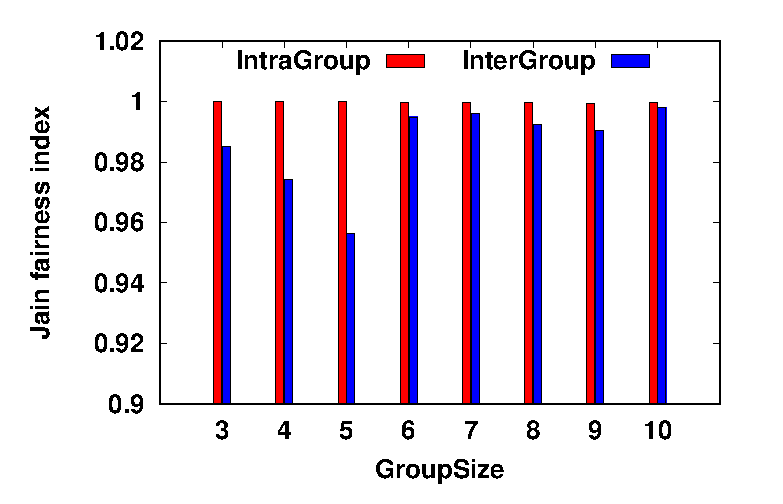
\includegraphics[width=0.49\linewidth]{img/grpbasic/grpsz_fairness}
		}
	\end{center}
	\caption{\label{fig:grpsz}Effect of Coalition Size}
\end{figure*}

One of the major objectives of \textit{CaliDASH} is to reduce the usage of streaming server when multiple co-located streaming players play the same live video. In Fig.~\ref{fig:cdnuploaded}, we plot the streaming server usage by different baselines in terms of the total bytes downloaded from the streaming server and the number of video segments directly downloaded from the streaming server. We observe that that the streaming server usages by DHT is lowest. In the case of FLSD, players are bounded to receive data from its group only, while in case of DHT, a player can share segments with as many players as possible. The standalone players need to download all the segments directly from the server. Therefore, we observe a performance trade-off here -- FLSD significantly improves the QoE performance while having little increase in the streaming server load. In a nutshell, the proposed approach makes a balance between the QoE and streaming server load during the peer-assisted live video streaming.  
%Fig.~\ref{fig:avgBitrate}, \ref{fig:avgBitrateVar}, \ref{fig:Stall_Time} and \ref{fig:QoE} we report the general result we found from our experiment. Fig.~\ref{fig:QoE} is a plot of Quality of Experience. We calculate QoE using the Equation~\ref{eqn:QoE}. In the equation, $\alpha$ is the quality factor and $\beta$ and $\gamma$ are smoothness penalty and stall penalty.
%
%
%
%According to Fig.\ref{fig:avgBitrate} performance of BOLA very low and most of the players played in lower quality. BOLA is very conservative about the bitrate and very much concerned about the rebuffering time. Pensieve and MPC improved the video quality compared to the BOLA by utilising reinforcement learning and deep inspection respectively. DHT is the first system which uses the knowledge of existing players in the network. So, it improves an average video quality compared to ABR. However, FLSD clustered the players and played video in sync. In Fig.~\ref{fig:avgBitratecmf}, it is clear that there are clusters of players who played video in almost equal quality. Average variation in video quality is higher for FLSD. However, it is higher because it played in the video in high quality. A slight change in the quality incurs high variation.
%\begin{figure}[h]
%\captionsetup[subfigure]{}
%\begin{center}
%	\subfloat[\label{fig:benfit_bitrate} Benefit in terms of average bitrate]{
%		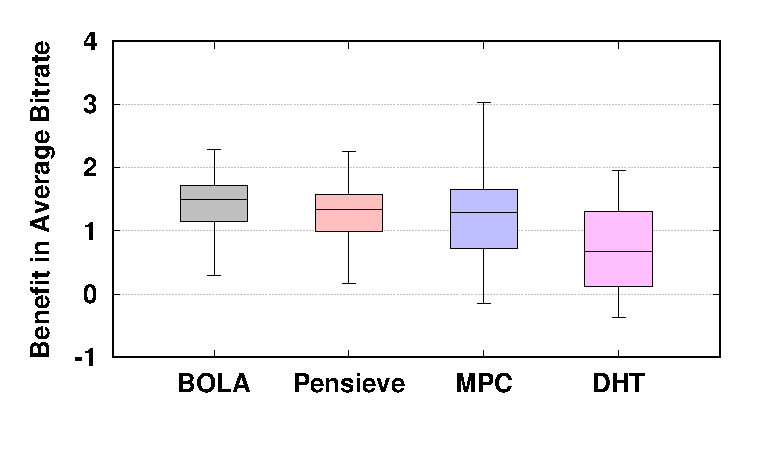
\includegraphics[width=0.49\linewidth]{img/grpbasic/benefit_bitrate_box_1}
%	}
%	\subfloat[\label{fig:benefit_qoe} Benefit in terms of QoE]{
%		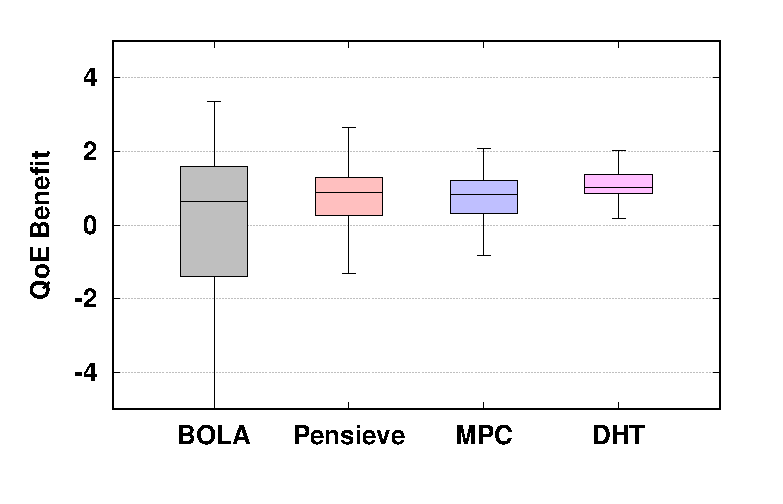
\includegraphics[width=0.49\linewidth]{img/grpbasic/benefit_qoe_box_1}
%	}
%\end{center}
%\caption{\label{fig:benefit}Per player benefit of using FLSD}
%\end{figure}





%\subsection{Benefit of using FLSD}
%In Fig.~\ref{fig:benefit}, we report the benefit of using FLSD instead of another streaming system for each player in the system. Here we plot only two metrics, i.e. average bitrate and QoE. To measure the benefit of using FLSD we need to keep the environment (i.e. network condition) of a player same for each ABR and reference network. It is possible for because our environment is simulated and the entire simulation state depends on the initial random variable\footnote{We use pseudo-random variable available in {\tt python numpy} library. It generates the same sequence of random numbers for the same seed/initial state.} state. However, it means that every time we run the experiment with the same environment, ABR and reference network, we get the same result. For this reason, we do not run the same experiment with the same environment, ABR and network. However, to measure the benefit of using FLSD instead of other ABR, we run an experiment on a large set of environments and reference network. We use Equation~\ref{eqn:benefit} to compute the benefit of a single player. Here $G_g$ is the metric for using FLSD and $G_o$ is the same metric for other ABR. We plot all the benefit as a box plot. Here benefit $Ben(S)==0$ means FLSD performed precisely the same as the other ABR. The positive and negative benefit means the better or worse performance of FLSD compared to other ABR.
%\begin{equation}
%Ben(S) = \frac{G_g - G_o}{|G_o|}
%\label{eqn:benefit}
%\end{equation}
%From Fig.~\ref{fig:benefit}, we can see that most of the player in the experiments gain some forms of benefit in terms of average playback quality as well as the QoE. The slight degradation in the benefit in terms of QoE with compared to BOLA. We have already seen in the Fig.\ref{fig:QoE} that QoE of BOLA is very high although the average quality is low because of its very low stall time. However, the overall performance of FLSD is higher than any other existing ABR or systems.
%\subsection{Effect of group size}
In all the previous experiments, we have fixed the maximum coalition size to 4 players. Here we check the effect of the increasing the coalition size. Fig.~\ref{fig:grp_qoe} and Fig.~\ref{fig:grp_download} shows the impact of different coalition sizes on the overall QoE and the total amount of data downloaded from the streaming server, respectively. We observe that a large coalition size provides better QoE because it gives more time to download a segment. However, in the case of a large coalition, every player has to upload more data to the other members of the coalition, which incurs an additional overhead.
%\subsection{Fairness}
In collaborative scenario, fairness among the members is an important metric. In our evaluation, we measure the fairness among the coalition members using Jain fairness index on QoE among the players \cite{jain1999throughput}. We measure the fairness among players in two categories, i) intra-coalition fairness (fairness among the coalition members of a coalition) and ii)inter-coalition fairness (fairness among the coalitions). The results are reported in Fig.~\ref{fig:grp_fairness}. We have computed fairness for seven different coalition sizes. Here we observe that the intra-coalition fairness index is always close to 1, which indicates good fairness. However, inter-coalition fairness is not very high as different coalitions can play video in different video quality which has a major contribution to the overall QoE. 
%From this result, we can conclude that FLSD is fair.
